\documentclass[11pt,a4paper]{article}

\usepackage{fullpage}
\usepackage{hyperref}
\usepackage{graphicx}
\usepackage{enumerate}
\usepackage{tikz}
\usepackage[bottom]{footmisc}
\usetikzlibrary{shapes, arrows, positioning, fit, backgrounds}
\usepackage{color}
\definecolor{pblue}{rgb}{0.13,0.13,1}
\usepackage{listings}
\lstset{language=Java,
		keywordstyle=\color{pblue},
		 breaklines=true,
		 basicstyle=\small,
		 tabsize=2
}
\usepackage{fancyhdr}
\pagestyle{fancy}
\fancyhf{}

\renewcommand{\headrulewidth}{0pt}
\renewcommand{\footrulewidth}{0pt}

\fancypagestyle{firstpagefooter} {
	\lfoot{\tiny{Version: 02.12.2017}}
	\cfoot{}
	\rfoot{\thepage}
	
}

\lfoot{Name: Simon Haefeli , Legi: 13-918-107}
\rfoot{\thepage}

\begin{document}

\title{Advanced Systems Lab Report\\ \normalsize{Autumn Semester 2017}}
\author{Name: Simon Haefeli\\Legi: 13-918-107}
\date{
	\vspace{4cm}
	\textbf{Grading} \\
	\vspace{0.5cm}
	\begin{tabular}{|c|c|}
		\hline  \textbf{Section} & \textbf{Points} \\
		\hline  1                &                 \\ 
		\hline  2                &                 \\ 
		\hline  3                &                 \\ 
		\hline  4                &                 \\ 
		\hline  5                &                 \\ 
		\hline  6                &                 \\ 
		\hline  7                &                 \\ 
		\hline \hline Total      &                 \\
		\hline 
	\end{tabular} 
}
\maketitle
\thispagestyle{firstpagefooter}

\newpage


\section{System Overview}
\subsection{Abstract}
This project consisted of designing, implementing and evaluating the performance of a key-value store network system. We added a so called middleware between the memtier benchmark clients and the memcached servers that was able to forward the requests and answers and do some processing for certain particular requests. In this report, we are first discussing the way the middleware has been implemented, analyze results of different experiments and finally modelling our system. 
\subsection{General design and implementation particularities}
Even though the general structure of the middleware was clearly defined, the components of the middlware asked for some important design choices. Here follow a small overview of the different implementation choices. 

\begin{center}
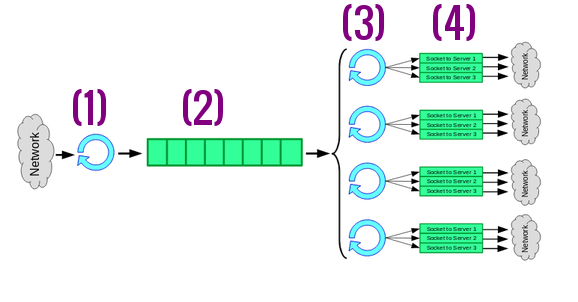
\includegraphics[scale=0.7]{baseIm.png}
\end{center}
\begin{enumerate}[ {(}1{)} ]
\item The net thread is the thread that accepts connections from the clients, and reads the incoming requests to put them in the request queue (2). The \textit{Java.nio} (non-blocking IO) package was used to achieve this purpose: A \textit{ServerSocketChannel} was used as a welcome socket to accept connections from the clients by creating for each client a \textit{SocketChannel}, and a \textit{Selector} was used to iterate over the the sockets (the connection sockets and the welcome socket) to find entering requests for the middleware or connection requests. Using the \textit{Java.nio} allows us not only to abstract the handling of a various number of connections, but also iterates over the client connections in an optimal way by using \textit{SelectionKeys}. 
\item The request queue is a java \textit{LinkedBlockingQueue}, which has the nice properties to be unbounded and beeing FCFS. Requests wait in this queue until a worker thread is free.   

\item The request queue and the worker threads are both managed by the java \textit{ThreadPoolExecutor}. The thread pool executor,which definition is: 
\begin{lstlisting}
	ThreadPoolExecutor(int corePoolSize, int maximumPoolSize, long keepAliveTime, TimeUnit unit, LinkedBlockingQueue workQueue)
\end{lstlisting} 
has a fixed number of worker threads by setting corePoolSize = maximumPoolSize. Putting a request into the queue or executing it, depending on the availability of the worker threads is beeing done by the same following instruction:
\begin{lstlisting}
	myThreadPoolExecutor.execute(Runnable command)
\end{lstlisting}
The \textit{ThreadPoolExecutor} will execute the command if a worker thread is available, or put it to the unbounded queue if not, which is exactly the expected behaviour.\footnote{https://docs.oracle.com/javase/7/docs/api/java/util/concurrent/ThreadPoolExecutor.html, part on "Queuing"}     
 
\item The connection sockets with the memcached servers are normal Java \textit{Socket}. Each worker thread opens a socket to each memcached server the first time it is beeing run and keeps it open until the middleware is stopped.  
\end{enumerate}

\subsection{Request handling}
We now want to look closer at the implementation of the middleware and how the pipeline looks like for a request beeing processed. The following flow chart illustrates this:
\\
\\\\
% Define block styles]
\tikzstyle{block} = [rectangle, draw, fill=blue!20, 
    text width=9em, text centered, rounded corners, minimum height=4em]
\tikzstyle{line} = [draw, -latex']
\tikzstyle{cloud} = [draw, ellipse,fill=red!20, node distance=3cm,
    minimum height=2em]   
\begin{tikzpicture}[node distance = 3cm, auto]
    % Place nodes
    \node [block] (RunMW) {\textbf{\underline{RunMW}} \\ \textit{main(): starts the mw}};
    \node [block, below=0.7cm of RunMW] (MyMiddleware) {\textbf{\underline{MyMiddleware}} \\ \textit{run(): reads the text from the socket and creates a prerequest}};
    \node [block, left=3cm of MyMiddleware, text width=8em] (Params) {\underline{Params} \\ inputs predefined parameters};
    \node [block, right=2cm of MyMiddleware] (PreRequest) {\textbf{\underline{PreRequest}} \\ \textit{PreRequest(): creates an object with the text and a starting time}};
    \node [block, below of=MyMiddleware] (QueueHandler) {\textbf{\underline{QueueHandler}} \\ \textit{putToQueue(): calls the threadPoolExecutor execute function on the Prerequest}};
    \node [block, left=3cm of QueueHandler, text width=11em] (StatisticsAggregator) {\textbf{\underline{StatisticsAggregator}} \\ \textit{run(): Gets statistics from different classes every time window, processes them and stores in the Statistics class}};
     \node [block, below of=StatisticsAggregator, text width=8em] (Statistics) {\underline{Statistics} \\ Contains the aggregated statistics};
      \node [block, below=1cm of QueueHandler] (RequestHandler) {\textbf{\underline{RequestHandler}} \\ \textit{run(): creates a Request to parse the PreRequest and calls the appropriate handling function}};
      \node [block, right=2cm of RequestHandler, text width=8em] (Request) {\textbf{\underline{Request}} \\ \textit{Request(): parses the text received from the client with the correct RequestType}};
      \node [block, above of=Request] (RequestType) {\underline{RequestType} \\ Contains the different request types};
      \node [cloud, below=0.8cm of RequestHandler] (HandleGet) {HandleGet()};
      \node [cloud, right=0.5cm of HandleGet] (HandleSet) {HandleSet()};
      \node [cloud, left=0.5cm of HandleGet] (HandleMGet) {HandleMGet()};
      
    % Draw edges
    \path [line] (RunMW) -- (MyMiddleware);
    \draw[>=latex,->] ([yshift= -5pt] PreRequest.west) -- ([yshift= -5pt] MyMiddleware.east);
    \draw[>=latex,<-] ([yshift= 5pt] PreRequest.west) -- ([yshift= 5pt] MyMiddleware.east);
  
    \path [line] (Params) -- (MyMiddleware);
    \path [line, dashed] (MyMiddleware) -- (StatisticsAggregator);
    \path [line, dashed] (QueueHandler) -- (StatisticsAggregator);
    \path [line, dashed] (RequestHandler) -- (StatisticsAggregator);
    \path [line] (StatisticsAggregator) -- (Statistics);
    \path [line] (MyMiddleware) -- (QueueHandler);
    \path [line] (QueueHandler) -- (RequestHandler);
    \draw[>=latex,->] ([yshift= 5pt] RequestHandler.east) -- ([yshift= 5pt] Request.west);
    \draw[>=latex,<-] ([yshift= -5pt] RequestHandler.east) -- ([yshift= -5pt] Request.west);
    \draw[>=latex,<-] ([xshift= 5pt] Request.north) -- ([xshift= 5pt] RequestType.south);
    \draw[>=latex,->] ([xshift= -5pt] Request.north) -- ([xshift= -5pt] RequestType.south);
    \path [line] (RequestHandler) -- (HandleMGet);
    \path [line] (RequestHandler) -- (HandleGet);
    \path [line] (RequestHandler) -- (HandleSet);
\end{tikzpicture}

\newpage

To make some correpondencies with the general structure of the middleware presented in section 1.2, we see that the \textit{MyMiddleware run()} function represents the net thread, the \textit{QueueHandler} class has a \textit{ThreadPoolExecutor} field that manages the request queue and the call of the worker thread, and that the \textit{RequestHandler run()} function represents one worker thread. We may also note that a PreRequest class is beeing created before putting the received message into the queue. This is to bind the message with a time, to be able to track the time a message spends in the queue. 
\\\\
At the end of the pipeline, the different requests are treated according to their type (get, set, or multi-get). In case of a set, the request is sent to all memcached servers sequentially, after what the worker thread waits for all the answers, also sequentially, as showed in the next line in the case of 3 memcached servers. 
\begin{lstlisting}
	1				send to server 1
	2				send to server 2
	3				send to server 3
	4				wait for answer 1 until received
	5				wait for answer 2 until received
	6				wait for answer 3 until received
	7				merge the answers and send back to client
\end{lstlisting}
The main drawback of this design is that if one of the server has a higher latency than the other ones, the worker thread might be waiting idle instead of starting to read the answers from the other servers. 
\\
In case of a get request, we simply forward the request to a given server. To decide which memcached server we send the request, we simply keep a static field in the \textit{RequestHandler} class which is shared accross the worker threads that keeps track of the last server to which we sent a get request. This variable is then beeing updated in a round-robin way. 
\\
In case of a multi-get, two cases are possible: In the non-sharded case, the request is simply beeing executed as a normal get. In the sharded case, the multi get is beeing splitted equally accross the different available memcached servers.   
\\\\
Finally, since we want the connections between the middleware and the servers to be open before running the experiments, we need to initialize these once for every worker thread. By defining the sockets in a \textit{ThreadLocal} in the \textit{RequestHandler} class, the initialization of the sockets will happen only the first time a worker thread is beeing called. That's why every thread is called once during the initialization phase of the middleware, by executing number of worker threads "init" requests, which are fake requests that don't need any special handling.\footnote{According to the javadoc of the ThreadPoolExecutor class, "When a new task is submitted in method execute(java.lang.Runnable), and fewer than corePoolSize threads are running, a new thread is created to handle the request, even if other worker threads are idle". And that's why it is enough to run corePoolSize number of requests to have them run all once and thus initialized their sockets.} 

\subsection{Statistics gathering}
Statistics have to be made in different classes accross the middleware, either a count (number of gets, number of sets,...), or an average (queue length, time in queue,...). These statistics are beeing stored in static atomic fields in the respective classes, that can be gotten from the \textit{StatisticsAggregator} class, which is a \textit{Runnable} called every second, the first time at initialization of the middleware. These statistics are then collected every given time window, averaged and stored in the \textit{Statistics} class. This process is beeing illustrated in the next figure:
\\
% Define block styles]
\tikzstyle{block} = [rectangle, draw, fill=green!20, 
    text width=36em, text centered, rounded corners, minimum height=4em]
\tikzstyle{line} = [draw, -latex'] 
\begin{tikzpicture}[node distance = 3cm, auto]
    % Place nodes
      \node [block, text width=36em] (StatisticsAggregator) {\textbf{\underline{StatisticsAggregator}} \\\begin{lstlisting}
	public void run(){
		int timesInQueue = Requesthandler.timesInQueue.getAndSet(0);
		int timesInQueueCount = Requesthandler.timesInQueueCount.getAndSet(0);
		Statistics.queueTimes.add(timesInQueue/timesInQueueCount);
	}
\end{lstlisting}};
    \node [block,text width=31em, below=6cm of StatisticsAggregator.west, anchor=west] (RequestHandler) {\textbf{\underline{RequestHandler}} \\\begin{lstlisting}
	public static AtomicInteger timesInQueue = 0;
	public static AtomicInteger timesInQueueCount = 0;
	public void handleRequest(request){
		ellapsedTime = System.nanoTime()-request.startTime;
		timesInQueue.getAndAdd(ellapsedTime);
		timesInQueueCount.getAndIncrement();
	}
\end{lstlisting}};
    \node [block, right=9cm of RequestHandler.north, anchor=north, text width = 10em] (Statistics) {\underline{Statistics} \\\begin{lstlisting}
	List<Integer> queueTimes;
\end{lstlisting}};
      
    % Draw edges
    \path [line] (StatisticsAggregator) -| (Statistics);
    \draw[>=latex,->] ([xshift= -5pt] RequestHandler.north) -- ([xshift= -5pt] StatisticsAggregator.south);
    \draw[>=latex,<-] ([xshift= 5pt] RequestHandler.north) -- ([xshift= 5pt] StatisticsAggregator.south);

\end{tikzpicture}
\\\\
The collected statistics in the \textit{Statistics} class are then beeing filtered, by removing the warm-up time (according to some experiments I made, the middlware needs around 10 seconds to get stable data) and the cool down time (1 second), and removing the zero values that are present before and after the significative values (zeros that occur because of the late start of a memtier client for example or an early stop). 
\\
Finally, when the middleware is shut down, the average and standart deviation of every statistic is beeing computed and printed to a file. Depending on the experiment, we sometimes also print all the values to construct histograms.
\newpage  
\section{Baseline without Middleware}
The goal of this experiment is to study how the system would perform without the middleware. This part is important to get a better idea of what the performance limitations of the memcached servers and the memtier benchmark clients are, so we can better judge of the impact of the middleware through the rest of the experiments. 

\subsection{One Server}

First, we want to analyze the performance evolution of the memcached server, and eventually find its upper-bound in terms of performance. To achieve this, we set up one single memcached server beeing queried by a various number of clients, for read-only and write-only workloads. More precisely, we are running experiments in the following configurations:
\begin{center}
	\scriptsize{
		\begin{tabular}{|l|c|}
			\hline Number of servers                & 1                        \\ 
			\hline Number of client machines        & 3                        \\ 
			\hline Instances of memtier per machine & 1                        \\ 
			\hline Threads per memtier instance     & 2                        \\
			\hline Virtual clients per thread       & [1..32]                  \\ 
			\hline Workload                         & Write-only and Read-only \\
			\hline 
		\end{tabular}
	} 
\end{center}

\subsubsection{Results and explanation}
For a read only workload, we obtain the following plots for the latency and the throughput, for one client machine (the plots are very similar than the ones of the other client machines):
\\
\begin{minipage}{0.5\linewidth}
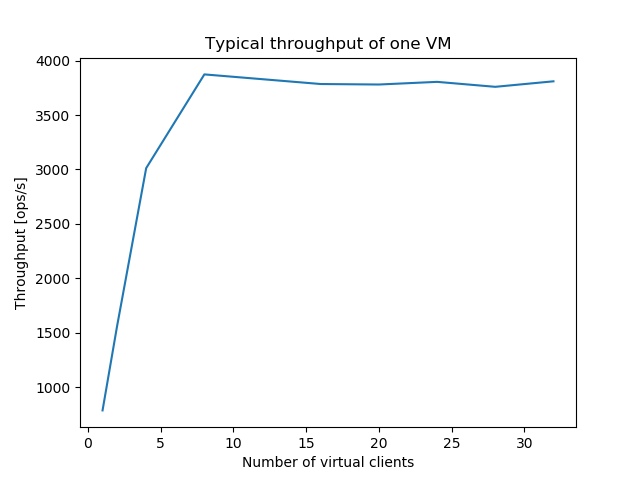
\includegraphics[width=\linewidth]{/home/simon/Documents/ETH/asl/asl-fall17-project/collectedStatFiles/Exp2/baseline1/readOneVMThroughput.png}
\end{minipage}
\hfill
\begin{minipage}{0.5\linewidth}
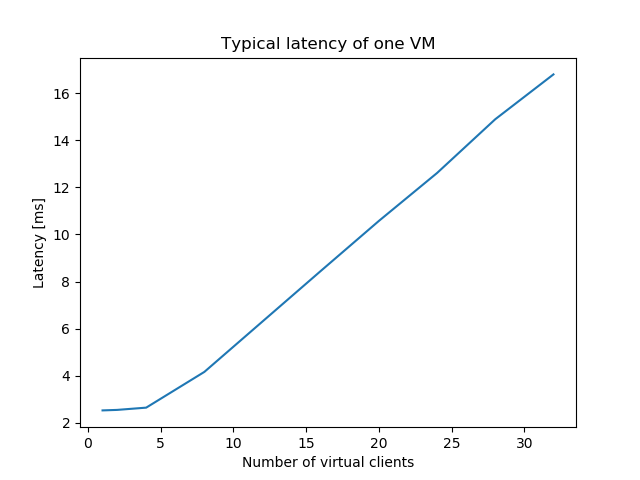
\includegraphics[width=\linewidth]{/home/simon/Documents/ETH/asl/asl-fall17-project/collectedStatFiles/Exp2/baseline1/readOneVMLatency.png}
\end{minipage}
\\\\
We notice that the maximum throughput is already obtained with 8 virtual clients per virtual machine and is then stable as we let the number of clients grow. This is, the memcached server starts to saturate when 3 VM with 2 threads and 8 virtual clients are querying a single server simultaneously. It is important to mention here that it is nearly impossible to over-saturate a server due to the way the memtier benchmark work: since we always run the clients with the default \textit{--pipeline=1} argument, every CPM\footnote{virtual client per memtier, see project description} will wait for an answer to come back before sending another request.
\\
For the latency, we clearly see that is inversely proportionnal to the througput (we distinguish three different slopes on both graphs). In the phase When the number of virtual clients grows at a constant rate (number of virtual clients getting bigger than 8), the throughput also gets constant. The reason why the throughput doesn't drop but stays at approximately 4000 operations/second is because the higher latency is compensated by a higher number of virtual clients to keep the throughput constant. Also, as a sanity check, we can evaluate the interactive law. Knowing that the interactive law is : \[ request time (w) = \frac{number of clients (N)}{throughput (X)}\], that for example at 8 virtual clients with two threads in the memtier client, N = 16 and the throughput X is approximately 3800 ops/sec,it gives us a reponse time of 4.2ms, which perfectly corresponds. This sanity check also works with the resting results of this experiment. 
\\
For a write-only workload, we obtain the following results:
\\
\begin{minipage}{0.5\linewidth}
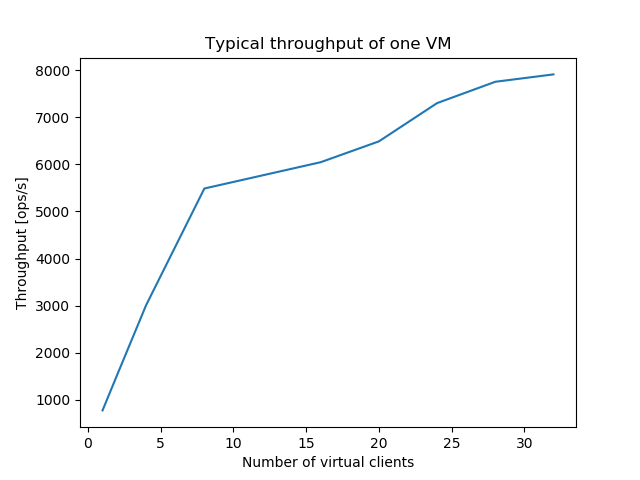
\includegraphics[width=\linewidth]{/home/simon/Documents/ETH/asl/asl-fall17-project/collectedStatFiles/Exp2/baseline1/writeOneVMThroughput.png}
\end{minipage}
\hfill
\begin{minipage}{0.5\linewidth}
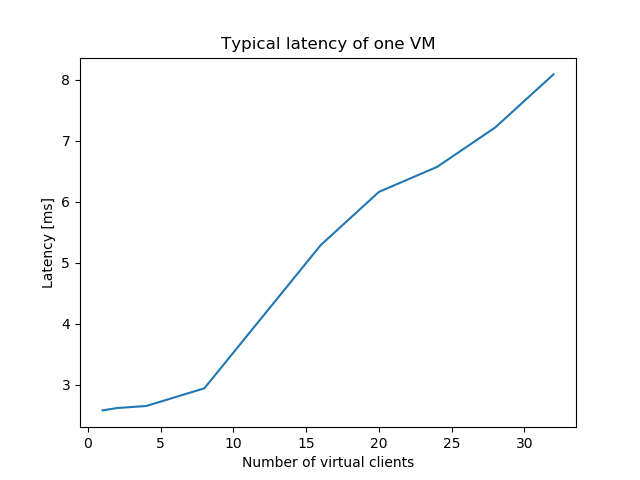
\includegraphics[width=\linewidth]{/home/simon/Documents/ETH/asl/asl-fall17-project/collectedStatFiles/Exp2/baseline1/writeOneVMLatency.png}
\end{minipage}
\\\\\\
For this workload, we note that we barely reach a saturated memcached server with 32 virtual clients, even if there is a clear drop in the growth of the throughput at 8 virtual clients. For write-only, the same observations apply as for the read-only workload. 
\\\\
However, we note a maximum throughput twice as high for sets than for gets, with a maximum latency twice as small. The differnce size of the messages beeing sent back and forth between the clients and the servers may not be the main factor, since for a get the messages are: 
\begin{lstlisting}
	request: get memtier-9999, 		answer: value memtier-9999 XXXXXX
\end{lstlisting}
and for the set they are:
\begin{lstlisting}
	request: set memtier-9999  0 10000 1024 XXXXX,	answer:  STORED
\end{lstlisting}
which are quite the same length. This implies that memcached is either storing values faster than getting values, either send the \textit{STORED} message back before starting the write operation, either having poorer performance than memtier benchmark when writting big messages to the connection sockets, or a combination of these factors. For this report, we will just keep in mind that the achieved throughput is higher with a write-only workload.
   
\subsection{Two Servers}

Now we are increasing the number of servers and putting a single client machine with a single thread to measure the see the performance limitations of the memtier clients with the following configurations:

\begin{center}
	\scriptsize{
		\begin{tabular}{|l|c|}
			\hline Number of servers                & 2                        \\ 
			\hline Number of client machines        & 1                        \\ 
			\hline Instances of memtier per machine & 2                        \\ 
			\hline Threads per memtier instance     & 1                        \\
			\hline Virtual clients per thread       & [1..32]                  \\ 
			\hline Workload                         & Write-only and Read-only \\
			\hline 
		\end{tabular}
	} 
\end{center}

\subsubsection{Results and explanation}
For a read-only workload, we obtain the following plots:
\\
\begin{minipage}{0.5\linewidth}
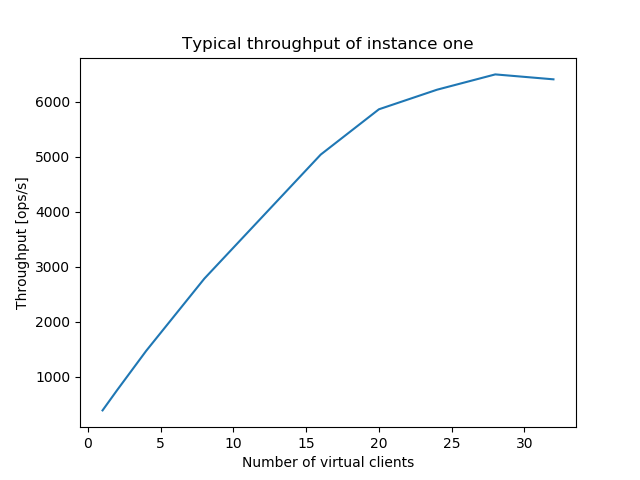
\includegraphics[width=\linewidth]{/home/simon/Documents/ETH/asl/asl-fall17-project/collectedStatFiles/Exp2/baseline2/readInst1Throughput.png}
\end{minipage}
\hfill
\begin{minipage}{0.5\linewidth}
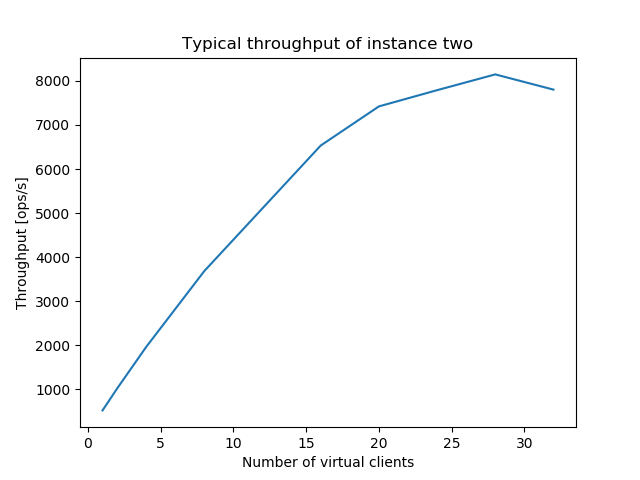
\includegraphics[width=\linewidth]{/home/simon/Documents/ETH/asl/asl-fall17-project/collectedStatFiles/Exp2/baseline2/readInst2Throughput.png}
\end{minipage}
\\\\
Remember that the client machine has two instances each connected to a different memcached server. It is important to notice at this point that the maximal throughput achieved by the two instances are not equal. As shown on the next figures, this is because the latency is higher for one of the two servers, which may be because of their geographic location (The server located further away from the client machine results in a higher latency).
\begin{minipage}{0.5\linewidth}
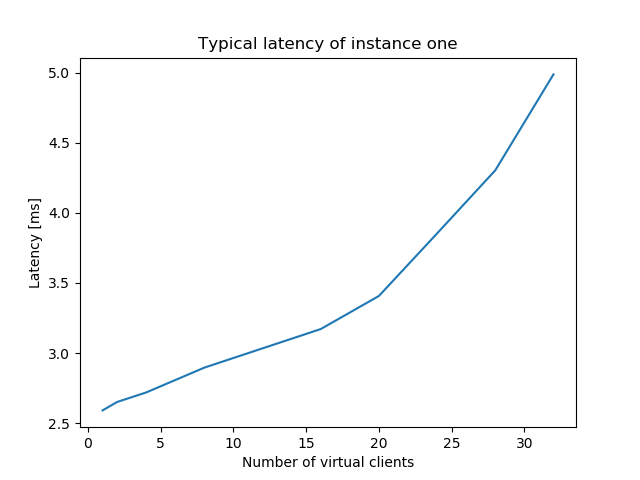
\includegraphics[width=\linewidth]{/home/simon/Documents/ETH/asl/asl-fall17-project/collectedStatFiles/Exp2/baseline2/readInst1Latency.png}
\end{minipage}
\hfill
\begin{minipage}{0.5\linewidth}
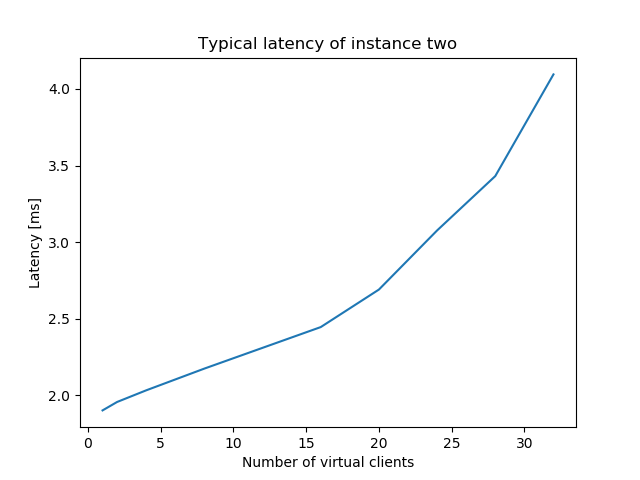
\includegraphics[width=\linewidth]{/home/simon/Documents/ETH/asl/asl-fall17-project/collectedStatFiles/Exp2/baseline2/readInst2Latency.png}
\end{minipage}
\\\\
For a write-only workload, we obtain for the server with higher througput similar plots for throughput and latency than for a read-only workload:
\\
\begin{minipage}{0.5\linewidth}
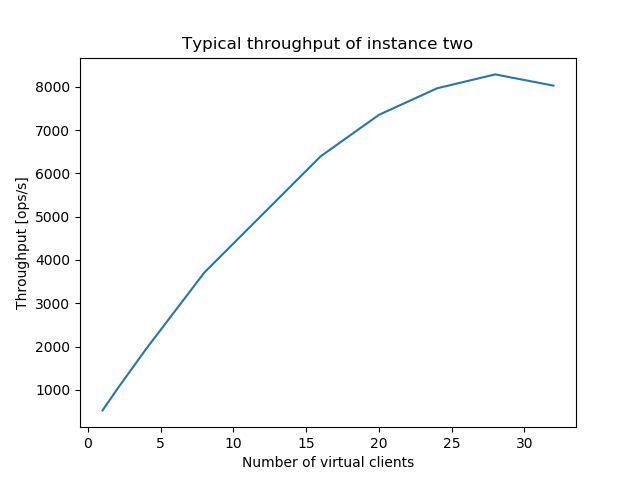
\includegraphics[width=\linewidth]{/home/simon/Documents/ETH/asl/asl-fall17-project/collectedStatFiles/Exp2/baseline2/writeInst2Throughput.png}
\end{minipage}
\hfill
\begin{minipage}{0.5\linewidth}
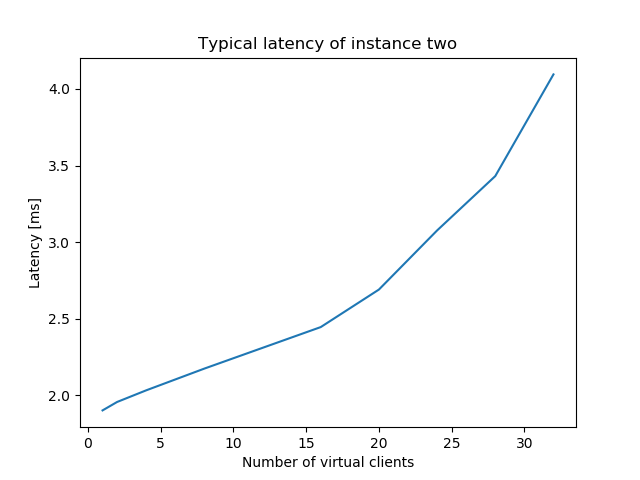
\includegraphics[width=\linewidth]{/home/simon/Documents/ETH/asl/asl-fall17-project/collectedStatFiles/Exp2/baseline2/writeInst2Latency.png}
\end{minipage}
\\
\\
We see that the system starts to saturate for the two workloads when reaching 28 virtual clients per thread, with a maximum throughput of around 8000 operations per second for the instance with higher throughput.  
We also note that contrary to the last experiment with a single server, the throughput for write and read are similar. This proves for the last experiment, that the memcached server saturates under a high workload, but tends to be more scalable for get-only operations. On the other hand, a single client machine cannot produce a higher throughput than 8000 operations per second, for read and for write.   
\subsection{Summary}


Based on the experiments, we are now able to fill the table with the maximal throughputs for different configurations. To make the results suitable for comparison with the rest of the experiments, we sum up the throughputs observed on the different client machines. For the experiment with a single memtier client, we use the results of both instances to give a lower and upper bound (separated by a "/"). 

\begin{center}
	{Maximum throughput meaasured on one VM}
	\begin{tabular}{|l|p{2cm}|p{2cm}|p{4cm}|}
		\hline                        & Read-only workload & Write-only workload & Configuration gives max. throughput \\ 
		\hline One memcached server   &11289                    &23836                     &8 VC for read-only, 32  VC for write-only                                     \\ 
		\hline One load generating VM &6498/8146                    &6558/8287                     &28 VC                                     \\ 
		\hline 
	\end{tabular}
\end{center}
As explained in the previous sections, the key take-aways this experiment are the following:

\begin{itemize}
\item The achieved throughput by the memtier clients and even instances may vary: because of the geographic positions of the clients or other factors. 
\item The memcached servers saturate faster for a read-only workload. For a write-only workload, the throughput can be twice as high and is limited by the performance of the memtier clients. 
\item The numbers of the first line in the table represent the max throughput a memcached server can achieve, as the second line represents the maximum workload a memtier client can achieve. 
\end{itemize}
\newpage

\section{Baseline with Middleware}

In this set of experiments we want to take a closer look on the effect of the middleware on the system. For this purpose, we are running experiments with different workloads, a different number of worker threads in the middleware, and one or two middlewares. This will show us in what way the middleware influences the results found during experiment two. 


\subsection{One Middleware}

We start the experiment by connecting a single client machine to the middleware and one memcached server, for different workloads and number of worker threads: 

\begin{center}
	\scriptsize{
		\begin{tabular}{|l|c|}
			\hline Number of servers                & 1                        \\ 
			\hline Number of client machines        & 1                        \\ 
			\hline Instances of memtier per machine & 1                        \\ 
			\hline Threads per memtier instance     & 2                        \\
			\hline Virtual clients per thread       & [1..32]                  \\ 
			\hline Workload                         & Write-only and Read-only \\
			\hline Number of middlewares            & 1                        \\
			\hline Worker threads per middleware    & [8..64]                  \\
			\hline 
		\end{tabular}
	} 
\end{center}

\subsubsection{Results and explanation}

The throughput and the response time for a read-only workload measured on the middleware give the following plots (the plots for write-only are the same):

\begin{center}
\includegraphics[scale=0.8]{/home/simon/Documents/ETH/asl/asl-fall17-project/collectedStatFiles/Exp3/part1/normal/statsMW/ratio0:1/rep1/throughput.png}
\end{center}
\begin{center}
\includegraphics[scale=0.8]{/home/simon/Documents/ETH/asl/asl-fall17-project/collectedStatFiles/Exp3/part1/normal/statsMW/ratio0:1/rep1/responseTime.png}
\end{center}

Note that the response time mesured is the addition of the service time and the waiting time in the queue, as showed by the two following plots. 
\\
\begin{minipage}{0.5\linewidth}
\includegraphics[width=\linewidth]{/home/simon/Documents/ETH/asl/asl-fall17-project/collectedStatFiles/Exp3/part1/normal/statsMW/ratio0:1/rep1/serviceTime.png}
\end{minipage}
\hfill
\begin{minipage}{0.5\linewidth}
\includegraphics[width=\linewidth]{/home/simon/Documents/ETH/asl/asl-fall17-project/collectedStatFiles/Exp3/part1/normal/statsMW/ratio0:1/rep1/timeInQueue.png}
\end{minipage}
\\
The service time of the middleware is extremely close to the time it takes to send and receive an answer from the memcached server (the difference can be neglected). Since the parsing times are very small compared to the answer time of memcached, the answer time and the service time are quasi equal. 
\\
The interactive law is also respected for the configurations where the maximum throughput is achieved. If we take for example 16 middleware worker threads and 32 virtual clients, we obtain N = 64, X = 6000, and thus w = 10 ms, which is not far from what we ploted (In reality, as we will see later, the time spent in the middleware, known as "think time" has also to be taken in account). 
\\
From the four of these plots, we see that the middleware is the bottleneck for a configuration with 8 and 16 middleware worker threads, since the throughput stays constant after respectively 8 and 16 virtual client and, as seen in the last experiment, the maximum throughput that can be achieved by memtier is higher than the throughputs achieved here. More precisely, the bottleneck in the middleware is the time a request spends in the queue, as shown by the strongly growing curve of the average time in queue for 8 worker threads for example. This strong growth is also correlated to the average queue length: as shown in the next figure, the queue length is growing with the time a request spends in queue, since the middleware has not enough thread available to execute the requests. 
\begin{center}
\includegraphics[scale=0.5]{/home/simon/Documents/ETH/asl/asl-fall17-project/collectedStatFiles/Exp3/part1/normal/statsMW/ratio0:1/rep1/queueLength.png}
\end{center}
As a sanity check, we also plot the latency and the throughput observed on the client:
\\
\begin{minipage}{0.5\linewidth}
\includegraphics[width=\linewidth]{/home/simon/Documents/ETH/asl/asl-fall17-project/collectedStatFiles/Exp3/part1/normal/statsClient/ratio0:1/rep1/throughput.png}
\end{minipage}
\hfill
\begin{minipage}{0.5\linewidth}
\includegraphics[width=\linewidth]{/home/simon/Documents/ETH/asl/asl-fall17-project/collectedStatFiles/Exp3/part1/normal/statsClient/ratio0:1/rep1/latency.png}
\end{minipage}
\\
There are two interesting points to notice: first, the throughput measured on the middleware is equal to the one measured on the memtier VM, which is due to the way memtier works. As explained in section 1, one memtier CPM doesn't send a new request until the last one has not been received. Secondly, the graph of the latency is similar as the one for the response time on the middleware, but shifted by 2ms on the y-axis, which is due to the travelling time between the middleware and the memtier client. 
\\
\\
As a last point, because we haven't reached a saturated middleware with 32 and 64 worker threads, we re-run the experiment with increased number of generating client VM number (2), to obtain the following results:
\\
\begin{minipage}{0.5\linewidth}
\includegraphics[width=\linewidth]{/home/simon/Documents/ETH/asl/asl-fall17-project/collectedStatFiles/Exp3/part1/bs/statsMWBottSearch/throughput.png}
\end{minipage}
\hfill
\begin{minipage}{0.5\linewidth}
\includegraphics[width=\linewidth]{/home/simon/Documents/ETH/asl/asl-fall17-project/collectedStatFiles/Exp3/part1/bs/statsMWBottSearch/timeInQueue.png}
\end{minipage}
\\
We note that by increasing the workload, we are able to saturate the middleware with 32 worker threads, again, dut to a slope change in the queuing time. For 64 worker threads, we are tending to reach a saturated state at around 11000 operations per second, which also corresponds to the maximum throughput a memcached server can achieve with a read-only workload. To make sure that the middleware becomes the bottleneck under high workload even with 64 worker threads, we have run all this experiment with a write-only workload also, and obtain for every configuration and every statistics the same plots. Seen that the maximum throughput of the memcached server under a write-only workload was around 20000 ops/second, we can conclude that the middleware will start to become the bottleneck under any configuration if the throughput is high enough. 
   
\subsection{Two Middlewares}

We continue the experiment by connecting one client VM with two instances of memtier to two different middlewares VMs and one memcached server:

\begin{center}
	\scriptsize{
		\begin{tabular}{|l|c|}
			\hline Number of servers                & 1                        \\ 
			\hline Number of client machines        & 1                        \\ 
			\hline Instances of memtier per machine & 2                        \\ 
			\hline Threads per memtier instance     & 1                        \\
			\hline Virtual clients per thread       & [1..32]                  \\ 
			\hline Workload                         & Write-only and Read-only \\
			\hline Number of middlewares            & 2                        \\
			\hline Worker threads per middleware    & [8..64]                  \\
			\hline 
		\end{tabular}
	} 
\end{center}
\subsubsection{Results and explanation}

We obtain the following plots for the throughput and response time measured on one middleware with similar plots for read-only and write-only workloads:
\\
\begin{minipage}{0.48\linewidth}
\includegraphics[width=\linewidth]{/home/simon/Documents/ETH/asl/asl-fall17-project/collectedStatFiles/Exp3/part2/normal/mw1/throughput.png}
\end{minipage}
\hfill
\begin{minipage}{0.48\linewidth}
\includegraphics[width=\linewidth]{/home/simon/Documents/ETH/asl/asl-fall17-project/collectedStatFiles/Exp3/part2/normal/mw1/responseTime.png}
\end{minipage}
\\
We directly notice that the difference of throughput and reponse time between different number of worker threads configuration isn't as significant as during the last experiment. As we will see on the next plots, this is because the high queuing time for a lower number of worker threads is compensated by a low service time and inversely. 
\\
\begin{minipage}{0.49\linewidth}
\includegraphics[width=\linewidth]{/home/simon/Documents/ETH/asl/asl-fall17-project/collectedStatFiles/Exp3/part2/normal/mw1/serviceTime.png}
\end{minipage}
\hfill
\begin{minipage}{0.49\linewidth}
\includegraphics[width=\linewidth]{/home/simon/Documents/ETH/asl/asl-fall17-project/collectedStatFiles/Exp3/part2/normal/mw1/timeInQueue.png}
\end{minipage}
\\\\ 
We should also take in consideration that the workload exerced on one middleware is halved compared to last experiment seen that there is only one thread per memtier instance and not two, which explains why the average time in queue for 8 worker threads only stats to grow faster after 16 virtual clients as opposed to 8. Furthermore, the throughput at saturation for 8 middleware threads is equal to the last experiment. 
Deducing from the previous experiment where we learnt that the bottleneck in the middleware is the queuing time, and the graphs above, the middleware hasn't reached its maximal throughput for the other configurations. 
\\\\
However, when we double the load on the middlewares, we can see that our middleware isn't the bottleneck of the experiment if we put a high number of worker thread, but the memcached server. If we remember the conclusions from the baseline without middleware, the read-only achieves a smaller maximal throughput than the write-only, and that's why we can suddently see a big difference in terms of throughput between the two workloads, since we showed during the last experiment that the middleware achieves the same performance for the two workloads when it is the bottleneck. This is shown by the following two graphs, the left one beeing a read-only workload and the right one a write-only workload (rep 2 mw1 used).   
\\
\begin{minipage}{0.5\linewidth}
\includegraphics[width=\linewidth]{/home/simon/Documents/ETH/asl/asl-fall17-project/collectedStatFiles/Exp3/part2/bs/statsMW01BottleneckSearch/ratio0/throughput.png}
\end{minipage}
\hfill
\begin{minipage}{0.5\linewidth}
\includegraphics[width=\linewidth]{/home/simon/Documents/ETH/asl/asl-fall17-project/collectedStatFiles/Exp3/part2/bs/statsMW01BottleneckSearch/ratio1/throughput.png}
\end{minipage}
\\\\
To confirm our claim, the calculation of the total throughput of the two middlewares on the single memcached server for a read and write only are (The two middlewares don't have the same throughput, but their statistics have exactly the same shape):
\\\textit{read : 4173+7043 = 11216 operations/second}
\\\textit{write : 5452+10753 = 16205 operations/second}
Hence, because the maximal throughput of a single memcached server for read-only workload was 11289, and 23836 for write-only, this proves that the memcached server is the bottleneck for this further experiment. This is, we can reach the memcached server upper-bound with a configuration with 64 worker thread and 2 connected middlewares. 



\subsection{Summary}
The maximum throughputs for different configurations are summarized in the following table. The throughputs are beeing added over all the VM as well for the middlewares than the clients. 

\begin{center}
	{Maximum throughput for one middleware.}
	\begin{tabular}{|l|p{2cm}|p{2cm}|p{2cm}|p{2cm}|}
		\hline                                & Throughput & Response time[ms] & Average time in queue[ms] & Miss rate \\ 
		\hline Reads: Measured on middleware  &10638           &6.69              &2.07                       &14\%           \\ 
		\hline Reads: Measured on clients     &10266            &12.25               &-                  &14\%           \\ 
		\hline Writes: Measured on middleware &10477            &7.17               &2.13                       &-      \\ 
		\hline Writes: Measured on clients    &10128            &12.63               &-                  &-       \\ 
		\hline 
	\end{tabular}
\end{center}

For this experiment, we take the average of the times since both middlewares don't have the same throughput. 
\begin{center}
	{Maximum throughput for two middlewares.}
	\begin{tabular}{|l|p{2cm}|p{2cm}|p{2cm}|p{2cm}|}
		\hline                                & Throughput & Response time & Average time in queue & Miss rate \\ 
		\hline Reads: Measured on middleware  &11216            &10.21               &1.09                       &0.1\%           \\
		\hline Reads: Measured on clients     & 11618            &12.246               &-                   &0.1\%           \\ 
		\hline Writes: Measured on middleware &16205            &6.305               &0.93                       &-       \\ 
		\hline Writes: Measured on clients    &16019            &8.915               &-                   &-       \\ 
		\hline 
	\end{tabular}
\end{center}

As explained in the previous sections, the key take-aways for this experiment are the following:

\begin{itemize}
\item The bottleneck of the middleware is the queuing time of the requests. When the number of worker threads is too low, this value tends to grow very fast.  
\item The same observation applies for a configuration with two middlewares. If the performance of the memcached servers and memtier benchmark clients were infinitely good, we would expect a performance as twice as high than for one middleware, since they are running independently. But this is not the case and could show that we can achieve the upper-bound of the memcached server with two middlewares. 
\end{itemize}
\newpage

\section{Throughput for Writes}

\subsection{Full System}

The purpose of this section is to assess the behaviour of the middleware with a write-only workloads and increased number of clients and servers.

\begin{center}
	\scriptsize{
		\begin{tabular}{|l|c|}
			\hline Number of servers                & 3          \\ 
			\hline Number of client machines        & 3          \\ 
			\hline Instances of memtier per machine & 2          \\ 
			\hline Threads per memtier instance     & 1          \\
			\hline Virtual clients per thread       & [1..32]    \\ 
			\hline Workload                         & Write-only \\
			\hline Number of middlewares            & 2          \\
			\hline Worker threads per middleware    & [8..64]    \\
			\hline 
		\end{tabular}
	} 
\end{center}

\subsubsection{Results and explanation}

The statistics of a single middleware have as expected the same shape than during last experiment, and are quasi equal between two middlewares. Hence, we plot here the total throughput of the two middlewares and the other statistics from one single middleware. 

\begin{center}
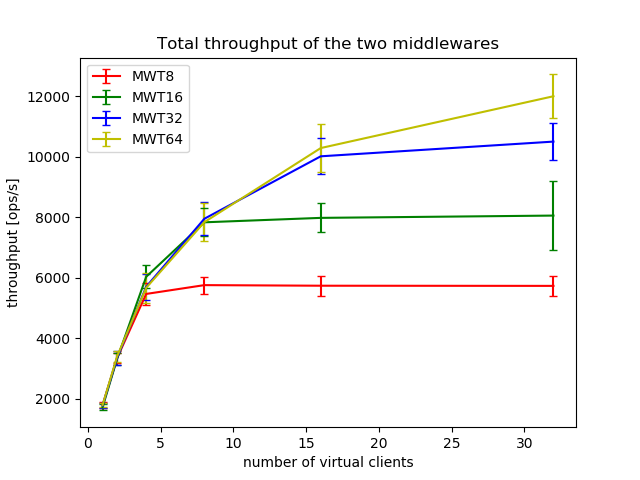
\includegraphics[scale=0.6]{/home/simon/Documents/ETH/asl/asl-fall17-project/collectedStatFiles/Exp4/totalThroughputM1and2/totalThroughput.png}
\end{center}
 \begin{center}
\includegraphics[scale=0.6]{/home/simon/Documents/ETH/asl/asl-fall17-project/collectedStatFiles/Exp4/statsMW1/responseTime.png}
\end{center}

The interactive law also holds for this case. If we take for example 32 worker threads at 16 virtual clients, we get N = 16*6 (since there are 3 clients putting workloads on these two middleware), X = 10000, we get w = 0.0096 = 9.6 ms, which is approximately correct. 
We further notice that the latency takes much higher values than during the last experiment, which is due to an increased workload from more clients. 
\\
We now want to get an insight on the service time compared to the queuing time.
\\
\begin{minipage}{0.5\linewidth}
\includegraphics[width=\linewidth]{/home/simon/Documents/ETH/asl/asl-fall17-project/collectedStatFiles/Exp4/statsMW1/serviceTime.png}
\end{minipage}
\hfill
\begin{minipage}{0.5\linewidth}
\includegraphics[width=\linewidth]{/home/simon/Documents/ETH/asl/asl-fall17-project/collectedStatFiles/Exp4/statsMW1/timeInQueue.png}
\end{minipage}
\\\\
We notcie that the service time stays constant after reaching a certain threshold. As we can see on the graph on the right, this is because of the time a request spents in queue. At one point, too many requests enter the middleware and can't be processed directly due to the number of available worker threads. We also that the service time is higher for an increased number of middleware threads, which is due to the workload beeing put on the memcached server. For a low number of worker threads, the service time stays low due to an under-saturated memcached server. 
A tradeoff between service time and average queuing is also to be seen: A higher number of worker threads will increase the load on the memcached server and increase its response time, whereas a too low number of middleware threads skyrockets the queuing time. This is why the gap between the response times (single graph above for response) is big for a low number of middleware threads and grows smaller when increasing the number of worker threads. 
\\
At last, we have a look to the average queue length in the middleware:
\begin{center}
\includegraphics[scale=0.5]{/home/simon/Documents/ETH/asl/asl-fall17-project/collectedStatFiles/Exp4/statsMW1/queueLength.png}
\end{center}
As said in the previous experiment, the average queue length follows the shape of the queuing time. A small calulation allows us to explain these numbers. 
If we consider our middleware with \textit{m} number of worker threads, an average queue length of \textit{L}, the service time beeing {s}, and the waiting time in queue beeing \textit{T}, we can verify that: 
\[ T = \frac{L}{m}\cdot s \]
which is just the number of requests awaiting for a given worker thread times the average service time of one worker thread. For example, if we take m = 16, the number of virtual clients to be 32, we have L = 65, s = 4ms, and thus we obtain T = 16.25ms, which corresponds to what we measured. 
\subsection{Summary}
To fill in the summary table, we do the total throughput of the middlewares, and take one representative statistics for the rest. For the throughput derived from the MW response time we use the interactive law as showed at the start of this section. 
\begin{center}
	{Maximum throughput for the full system}
	\begin{tabular}{|l|p{1.5cm}|p{1.5cm}|p{1.5cm}|p{1.5cm}|}
		\hline                                            & WT=8 & WT=16 & WT=32 & WT=64 \\ 
		\hline Throughput (Middleware)                    &5734      &8060       &10507       &12008       \\ 
		\hline Throughput (Derived from MW response time) &5485      &9142       &12000       &14906       \\ 
		\hline Throughput (Client)                        &5769      &8438       &10384       &11791       \\ 
		\hline Average time in queue[ms]                      &31.2      &18.3       &10.0      &3.4       \\ 
		\hline Average length of queue                    &84      &72       &47       &19       \\ 
		\hline Average time waiting for memcached[ms]         &2.9      &3.9       &6.1       &9.3       \\ 
		\hline 
	\end{tabular}
\end{center}

The key take-aways for this experiment are the following: 
\begin{itemize}
\item There exists a tradeoff between the queuing time and the time waiting for memcached: The higher the number of worker threads is, the higher the load on the memcached servers is, but the lower the queuing time becomes and inversely
\item We could apply a simple law that links the service time, the number of worker threads, the length of the queue and the queuing time, as well as the interactive law. 
\end{itemize}
\newpage

\section{Gets and Multi-gets}

In this set of experiments we will have a closer look to the behaviour of the system with get and multi-get requests. First, the sharded case, where the middleware splits the requests among the servers, and secondly the non-sharded case, where the request is handled as a normal get. 

\subsection{Sharded Case}
The memtier worklad is adapted so that memtier sends one set alternated with one multi get of the key-size we want. Also, we use 64 middleware threads to achieve maximum throughput. 

\begin{center}
	\scriptsize{
		\begin{tabular}{|l|c|}
			\hline Number of servers                & 3                       \\ 
			\hline Number of client machines        & 3                       \\ 
			\hline Instances of memtier per machine & 2                       \\ 
			\hline Threads per memtier instance     & 1                       \\
			\hline Virtual clients per thread       & 2     		            \\ 
			\hline Workload                         & [1:1, 1:3, 1:6, 1:9]           \\
			\hline Multi-Get behavior               & Sharded                \\
			\hline Multi-Get size                   & [1, 3, 6, 9]                  \\
			\hline Number of middlewares            & 2                       \\
			\hline Worker threads per middleware    & 64 \\
			\hline 
		\end{tabular}
	} 
\end{center}

\subsubsection{Results and explanations}
First, we analyze a couple of statistics on the middleware to understand its behaviour. The throughput and the service time in the middleware are plotted:
\\
\begin{minipage}{0.5\linewidth}
\includegraphics[width=\linewidth]{/home/simon/Documents/ETH/asl/asl-fall17-project/collectedStatFiles/Exp5/statsMW1//shardedtrue/serviceTime.png}
\end{minipage}
\hfill
\begin{minipage}{0.5\linewidth}
\includegraphics[width=\linewidth]{/home/simon/Documents/ETH/asl/asl-fall17-project/collectedStatFiles/Exp5/statsMW1//shardedtrue/throughput.png}
\end{minipage}
\\\\
We observe that the service time increases with the key size, which is normal since the processing the middlware has to do for different key sizes is approximately equivalent, but the time taken by the server to process the request and sending the packet back is higher for a bigger key amount. For the sharded case, we know that the middleware has to split the requests into different servers, which may cause a bigger processing time. However, this additional processing time can be neglected as shown by the following graphics (The left one represents the total time a requests spents in the multi get handling, whereas the right graphics shows the wating time for memcached in the multi get handling). In fact the differences between the two is in micro seconds. 
\\
\begin{minipage}{0.5\linewidth}
\includegraphics[width=\linewidth]{/home/simon/Documents/ETH/asl/asl-fall17-project/collectedStatFiles/Exp5/statsMW1//shardedtrue/timesInMGet.png}
\end{minipage}
\hfill
\begin{minipage}{0.5\linewidth}
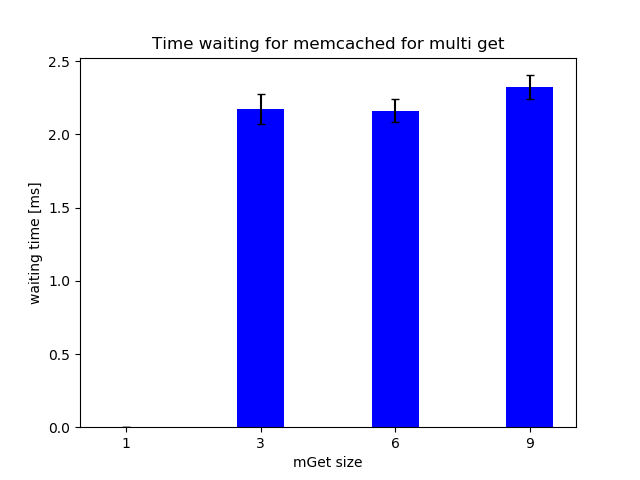
\includegraphics[width=\linewidth]{/home/simon/Documents/ETH/asl/asl-fall17-project/collectedStatFiles/Exp5/statsMW1//shardedtrue/timesInMGetMem.png}
\end{minipage}
\\\\
Two comments have to be made regarding these graphs: first, we see that there is no statistics for a key size of 1, this is because a multi get with size one is handled as a get in the middleware and thus isn't part of the multi get statistics. Secondly, we observe that the time spent in the multi get handling is equivalent to the service time. This is because the parsing time of a request is still very small even if the size of the message grows.
\\
In the previous sections, we discovered that the time spent in the queue was the bottleneck of our system. However, in a multi get configuration this isn't the case any more, as showed by the following figure, which plots the time spent in queue:  
 \begin{center}
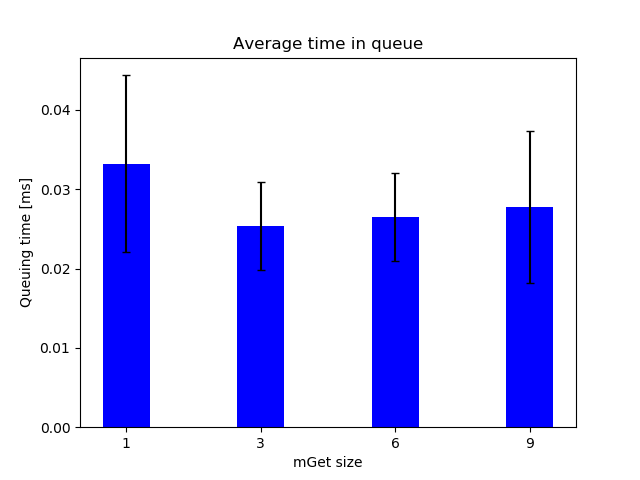
\includegraphics[scale=0.6]{/home/simon/Documents/ETH/asl/asl-fall17-project/collectedStatFiles/Exp5/statsMW1//shardedtrue/timesInQueue.png}
\end{center}


On the client side, a closer look is taken to the latency distribution of the requests. The plotted line represents the average lateny. The colors represent the percentage of the requests that are in a certain latency range. Hence, the top of a given color bar is a percentile. Thus, the top edge of the colors represent respectively the 25th, 50th, 75th, 90th and 99th percentile. 
  
 \begin{center}
\includegraphics[scale=0.7]{/home/simon/Documents/ETH/asl/asl-fall17-project/collectedStatFiles/Exp5/statsClient1//shardedTrue/latency.png}
\end{center}

We observe a similar behaviour than on the middleware with a small growth of the latency and that the values are clustered around the average as expected. A closer look at the distribution of the latency will be made at the end of this section. 

\subsection{Non-sharded Case}

The middleware is now beeing run in non-sharded mode. A multi-get request is therefor handled in the same way as a normal get. 

\begin{center}
	\scriptsize{
		\begin{tabular}{|l|c|}
			\hline Number of servers                & 3                       \\ 
			\hline Number of client machines        & 3                       \\ 
			\hline Instances of memtier per machine & 2                       \\ 
			\hline Threads per memtier instance     & 1                       \\
			\hline Virtual clients per thread       & 2                		 \\ 
			\hline Workload                         & [1:1, 1:3, 1:6, 1:9]             \\
			\hline Multi-Get behavior               & Non-Sharded             \\
			\hline Multi-Get size                   & [1..9]                  \\
			\hline Number of middlewares            & 2                       \\
			\hline Worker threads per middleware    & 64 \\
			\hline 
		\end{tabular}
	} 
\end{center}

\subsubsection{Results and explanations}

The results are extremely similar to the sharded case: we observe a growth of the latency with number of keys in the multi get. The latency as observed on the middleware and on the clients are shown as followed: 
\\
\begin{minipage}{0.5\linewidth}
\includegraphics[width=\linewidth]{/home/simon/Documents/ETH/asl/asl-fall17-project/collectedStatFiles/Exp5/statsMW1//shardedfalse/timesInMGet.png}
\end{minipage}
\hfill
\begin{minipage}{0.5\linewidth}
\includegraphics[width=\linewidth]{/home/simon/Documents/ETH/asl/asl-fall17-project/collectedStatFiles/Exp5/statsClient1/shardedFalse/latency.png}
\end{minipage}
\\\\
For this part, there is no surprise regarding the obtained results. As the key size grows, the memcached server needs more time to process the request and send the answer back, and thus we observe a growth of the latency. A detailed comparison between the sharded and non sharded case can be found under the two next sections. 

\subsection{Histogram}

The distribution of the latency as measured on the middleware and the client, for both sharded and non sharded case, for a key size of 6, gives the following plots (The histograms are constructed in a way so that bins having less than one request are not displayed):
\\
\begin{minipage}{0.5\linewidth}
\includegraphics[width=\linewidth]{/home/simon/Documents/ETH/asl/asl-fall17-project/collectedStatFiles/Exp5/statsClient1/shardedTrue/histogram6.png}
\end{minipage}
\hfill
\begin{minipage}{0.5\linewidth}
\includegraphics[width=\linewidth]{/home/simon/Documents/ETH/asl/asl-fall17-project/collectedStatFiles/Exp5/statsMW1/shardedtrue/HistMGetsize6.png}
\end{minipage}
\\
\\
\begin{minipage}{0.5\linewidth}
\includegraphics[width=\linewidth]{/home/simon/Documents/ETH/asl/asl-fall17-project/collectedStatFiles/Exp5/statsClient1/shardedFalse/histogram6.png}
\end{minipage}
\hfill
\begin{minipage}{0.5\linewidth}
\includegraphics[width=\linewidth]{/home/simon/Documents/ETH/asl/asl-fall17-project/collectedStatFiles/Exp5/statsMW1/shardedfalse/HistMGetsize6.png}
\end{minipage}


\subsection{Summary}

All the histograms seem to follow a gaussian distribution around a shifted mean. First, we notice that measured on the client is slightly higher than the one meaasured on the middleware, due to the travelling time between the middleware and the client. Secondly, more interesting, the latency is on average higher in the sharded case than in the non sharded case. 
\\
This can be explained by the followings: 
\begin{itemize}
\item The server performance is similar if it receives 2 keys in the get requests (in the sharded case with 3 servers) or 6 keys. This claim can be proved by looking at the graph in section 5.2, where we see that the difference of time spent in the multi get handling between 3 and 6 keys , i.e the waiting time for the memcached server, is very small. Hence, reducing the key size from 6 to 2 isn't significant enough to observe a significant differnce in latency. 
With a multi get key size of 9, the difference wouldn't have been significant either, by refering to the same graph again, since the request would have been split in sizes of 3. A major difference could have had been observed if we had a key size of n which overwhelms the server, whereas a size of n/3 doesn't. However, n=9 isn't enough to overwhelm the server, even with a very low miss ratio (1\%)
\item The way the middleware handles a multi-get request in the sharded mode isn't optimal. The pattern followed by the multi get handling is the same as the one for a set request, namely: 
\begin{lstlisting}
	1				prepare the splitted requests
	2				send to server 1
	3				send to server 2
	4				send to server 3
	5				wait for answer 1 until received
	6				wait for answer 2 until received
	7				wait for answer 3 until received
	8				merge the answers and send back to client
\end{lstlisting}
Like we discussed in the previous section, the point 1 is extremely efficient and can be neglected. However, waiting sequentially for an answer from a server can be bad if the response times are different as explained for set request. 
\end{itemize}  

\newpage
\section{2K Analysis}

\subsection{Parameters of the experiment}

\begin{center}
	\scriptsize{
		\begin{tabular}{|l|c|}
			\hline Number of servers                & 2 and 3                                     \\ 
			\hline Number of client machines        & 3                                           \\ 
			\hline Instances of memtier per machine & 2                                           \\ 
			\hline Threads per memtier instance     & 1                                           \\
			\hline Virtual clients per thread       & 32                                     \\ 
			\hline Workload                         & Write-only, Read-only, and 50-50-read-write \\
			\hline Number of middlewares            & 1 and 2                                     \\
			\hline Worker threads per middleware    & 8 and 32                                    \\
			\hline 
		\end{tabular}
	} 
\end{center}
\subsection{Results and explanation}

\section{Queuing Model (90 pts)}

Note that for queuing models it is enough to use the experimental results from the previous sections. It is, however, possible that the numbers you need are not only the ones in the figures we asked for, but also the internal measurements that you have obtained through instrumentation of your middleware.

\subsection{M/M/1}

Build queuing model based on Section 4 (write-only throughput) for each worker-thread configuration of the middleware. Use one M/M/1 queue to model your entire system. Motivate your choice of input parameters to the model. Explain for which experiments the predictions of the model match and for which they do not.

\subsection{M/M/m}

Build an M/M/m model based on Section 4, where each middleware worker thread is represented as one service.  Motivate your choice of input parameters to the model. Explain for which experiments the predictions of the model match and for which they do not.

\subsection{Network of Queues}

Based on Section 3, build a network of queues which simulates your system. Motivate the design of your network of queues and relate it wherever possible to a component of your system. Motivate your choice of input parameters for the different queues inside the network. Perform a detailed analysis of the utilization of each component and clearly state what the bottleneck of your system is. Explain for which experiments the predictions of the model match and for which they do not.

\end{document}
\grid
\grid
